\section{Method}
\label{sec:method}
-Choosing have to divide the different datatypes into abstract representations
-Creating the syntax for the abstract representations
--checking the soundness of the abstract representations
-Creating the semantics for the abstract representations
-implementing the abstract representations in kotlin
-through CLI it takes a database in the form af SQL queries and returns the abstract representation of the database after a set of operations have been performed on it defined by the user


\subsection{Example}\label{subsec:example}
To illustrate the method, we will use a simple example.
Consider a database with a single table, \texttt{account}, with two columns, \texttt{name} and \texttt{balance}.
For the program to work, we need to define the table for the database, this is shown in \autoref{fig:database-schema}.

\begin{figure}[htb!]
\begin{lstlisting}[language=SQL]
    CREATE TABLE account (
    name VARCHAR(50),
    balance INT
    );
\end{lstlisting}
\caption{SQL query for creating the table in the database}
\label{fig:database-schema}
\end{figure}

The UML diagram of the database schema is shown in \autoref{fig:uml-account}.

\begin{figure}[htb!]
    \centering
    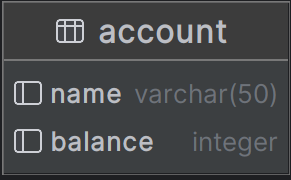
\includegraphics[width=0.25\textwidth]{figures/account.png}
    \caption{UML diagram of the abstract representation of the database schema}
    \label{fig:uml-account}
\end{figure}

The database has two operations, \texttt{insert} and \texttt{update}.
The \texttt{insert} operation inserts a new row into the table, i.e. a new user, and the \texttt{update} operation updates the balance of two accounts.
The SQL queries for the operations are shown in \autoref{lst:sql-queries} and \autoref{lst:sql-queries2}.
\begin{figure}
\begin{lstlisting}[language=SQL]
    INSERT INTO account (name, balance)
    VALUES (RANDOM_NAME, RANDOM_AMOUNT);
\end{lstlisting}
\label{lst:sql-queries}
\caption{SQL query for the insert operation}
\end{figure}

\begin{figure}[htb!]
\begin{lstlisting}[language=SQL]
    UPDATE account
    SET balance = CASE
    WHEN name = "name1" THEN balance - <amount_to_transfer>
    WHEN name = name2 THEN balance + <amount_to_transfer>
    ELSE balance
    END
    WHERE name IN (name1, name2);
\end{lstlisting}
\label{lst:sql-queries2}
\caption{SQL query for the update operation}
\end{figure}

Now the database schema and the operations are defined, we need to define the behavior of the operations.
The program that defines the behavior of the operations is shown in \autoref{lst:program}.
The program first checks if there are 2 or more accounts in the database, if not, it inserts a new account, with the \texttt{Insert} operation.
If there are more than two accounts, we try to transfer an amount from one account to another, that is the \texttt{Update} operation.

\begin{figure}[htb!]
\begin{lstlisting}
tansferamount:=?
formID:=R_ID
toID:=R_ID
if(transferAmount>0)
    <select(fromB,id,DISTINCT(id(AccBalance)),true,id),toID=AccID>
    <select(toB,id,DISTINCT(id(AccBalance)),true,id),toID=AccID>
    if(formB-transferAmount>0)
        <update(<AccBalance>,>fromB-transferAmount>),fromID=AccID>
        <update(<AccBalance>,>toB-transferAmount>),toID=AccID>


transF||newuser


B:=+
U:=?
<insert(U,B)> into (account)




while true do
    rand:=?
if rand<0
    then transF
    else newuser
\end{lstlisting}
\label{lst:program}
\caption{Program that defines the behavior of the operations}
\end{figure}

Now everything for the analysis is ready, we just need to define what the analysis should check for, this is defined by properties, that is defined by the LTL grammar on the attributes in the database.
The properties we want to check on the database are shown in \autoref{lst:properties}.
\begin{figure}[htb!]
\begin{lstlisting}
<>(transferAmount>0)
[](fromB-TransferAmount>0)
    \end{lstlisting}
\label{lst:properties}
\caption{Properties that the analysis check for}
\end{figure}

After inserting all the information into the program, the program makes a graph of system, which is shown in \autoref{fig:-program_graph}.

\begin{figure}[htb!]
    \centering
    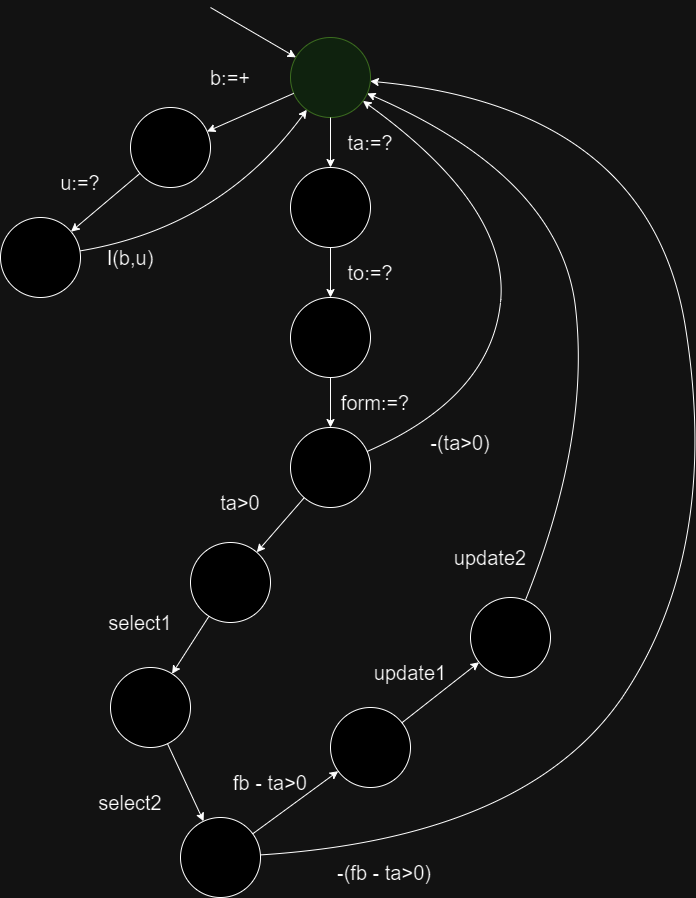
\includegraphics[width=0.5\textwidth]{figures/program_graph.png}
    \caption{Program graph of the system}
    \label{fig:-program_graph}
\end{figure}
\todo{Make the graph in tikz}